% Unique recruitment flowchart for the WWID analysis
% BBS among PWID, round II -- five Mozambican cities, 2023-2024
% Compile: pdflatex Figure_recruitment_flow.tex

\documentclass[11pt]{article}

\usepackage[T1]{fontenc}
\usepackage{lmodern}
\usepackage[margin=1cm,landscape,a4paper]{geometry}
\usepackage{tikz}
\usetikzlibrary{arrows.meta,calc}
\usepackage{array}
\usepackage{microtype}

\pagestyle{empty}
\setlength{\parindent}{0pt}
\renewcommand{\familydefault}{\sfdefault}

\newcommand{\N}[1]{\textbf{n = #1}}

\begin{document}

\begin{center}
{\large\bfseries Recruitment of PWID and selection of the WWID analytic sample}\\[2pt]
{\small Second-round Bio-Behavioral Survey (BBS-PWID II).
Maputo, Beira, Tete, Quelimane and Nampula, 2023--2024}
\end{center}
\vspace{1mm}

\begin{center}
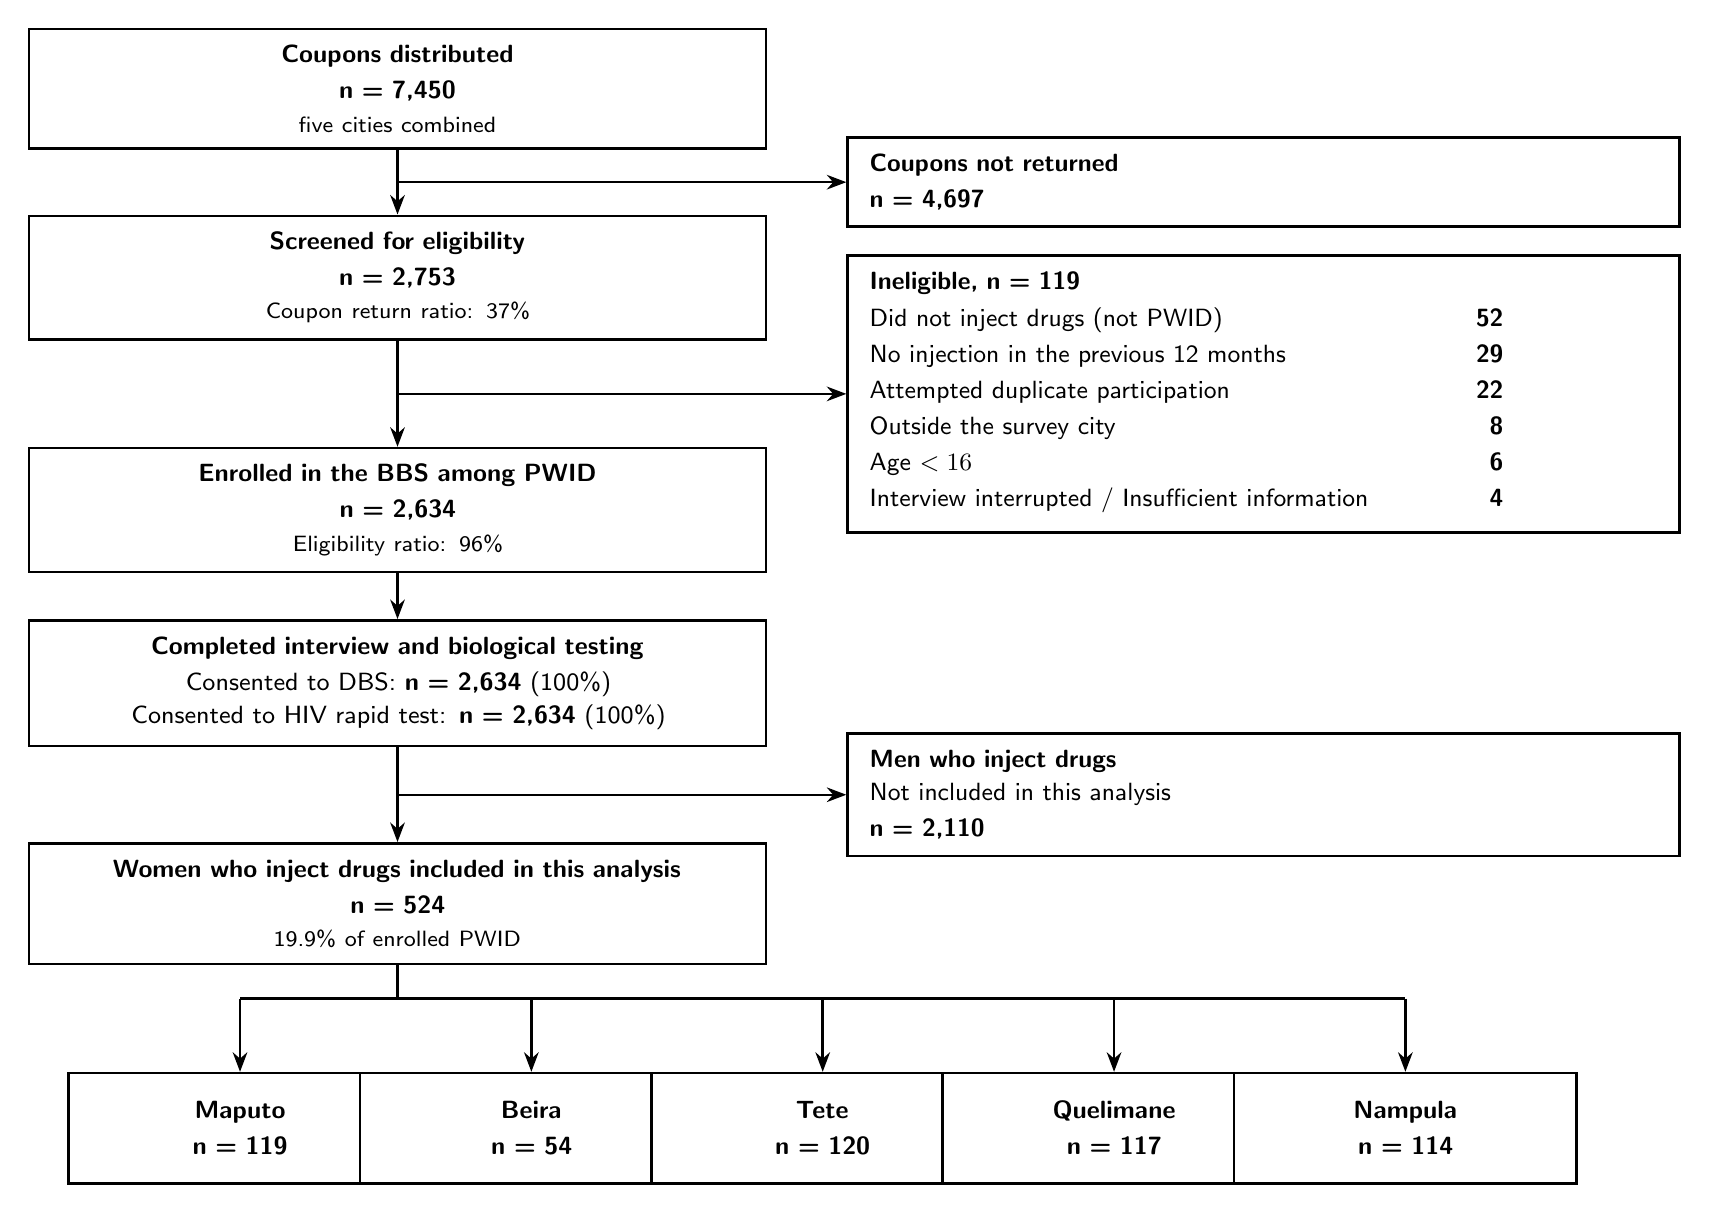
\begin{tikzpicture}[>=Stealth, x=1cm, y=1cm]

\tikzset{
  main/.style={
    draw,
    line width=0.9pt,
    fill=white,
    align=center,
    inner xsep=8pt,
    inner ysep=6pt,
    text width=88mm,
    rounded corners=0pt,
    font=\sffamily\small
  },
  excl/.style={
    draw,
    line width=0.9pt,
    fill=white,
    align=left,
    anchor=west,
    inner xsep=8pt,
    inner ysep=6pt,
    text width=100mm,
    minimum width=100mm,
    rounded corners=0pt,
    font=\sffamily\small
  },
  keep/.style={
    draw,
    line width=0.9pt,
    fill=white,
    align=center,
    inner xsep=8pt,
    inner ysep=6pt,
    text width=88mm,
    rounded corners=0pt,
    font=\sffamily\small
  },
  city/.style={
    draw,
    line width=0.9pt,
    fill=white,
    align=center,
    inner xsep=5pt,
    inner ysep=5pt,
    text width=40mm,
    minimum height=14mm,
    rounded corners=0pt,
    font=\sffamily\small
  }
}

% Left spine kept compact; tall ineligible box sits to the right
\node[main] (coupons) at (0,0) {%
  \textbf{Coupons distributed}\\[2pt]
  \N{7,450}\\[1pt]
  {\footnotesize five cities combined}};

\node[main] (screened) at (0,-2.40) {%
  \textbf{Screened for eligibility}\\[2pt]
  \N{2,753}\\[1pt]
  {\footnotesize Coupon return ratio: 37\%}};

\node[main] (enrolled) at (0,-5.35) {%
  \textbf{Enrolled in the BBS among PWID}\\[2pt]
  \N{2,634}\\[1pt]
  {\footnotesize Eligibility ratio: 96\%}};

\node[main] (consent) at (0,-7.55) {%
  \textbf{Completed interview and biological testing}\\[2pt]
  Consented to DBS: \N{2,634} (100\%)\\[1pt]
  Consented to HIV rapid test: \N{2,634} (100\%)};

\node[keep] (wwid) at (0,-10.35) {%
  \textbf{Women who inject drugs included in this analysis}\\[2pt]
  \N{524}\\[1pt]
  {\footnotesize 19.9\% of enrolled PWID}};

% Junctions on the blue spine: exclusions branch from these points
\coordinate (j-notret) at ($(coupons.south)!0.5!(screened.north)$);
\coordinate (j-inelig) at ($(screened.south)!0.5!(enrolled.north)$);
\coordinate (j-men)    at ($(consent.south)!0.5!(wwid.north)$);

\node[excl] (notret) at (5.7,0 |- j-notret) {%
  \textbf{Coupons not returned}\\[2pt]
  \N{4,697}};

\node[excl] (inelig) at (5.7,0 |- j-inelig) {%
  \textbf{Ineligible, n = 119}\\[3pt]
  \begin{tabular}{@{}p{72mm}@{\hspace{5mm}}r@{}}
  Did not inject drugs (not PWID) & \textbf{52} \\[2pt]
  No injection in the previous 12 months & \textbf{29} \\[2pt]
  Attempted duplicate participation & \textbf{22} \\[2pt]
  Outside the survey city & \textbf{8} \\[2pt]
  Age $< 16$ & \textbf{6} \\[2pt]
  Interview interrupted / Insufficient information & \textbf{4} \\
  \end{tabular}};

\node[excl] (men) at (5.7,0 |- j-men) {%
  \textbf{Men who inject drugs}\\[1pt]
  Not included in this analysis\\[2pt]
  \N{2,110}};

\node[city] (c1) at (-2.0,-13.20) {\textbf{Maputo}\\[2pt] \N{119}};
\node[city] (c2) at ( 1.7,-13.20) {\textbf{Beira}\\[2pt] \N{54}};
\node[city] (c3) at ( 5.4,-13.20) {\textbf{Tete}\\[2pt] \N{120}};
\node[city] (c4) at ( 9.1,-13.20) {\textbf{Quelimane}\\[2pt] \N{117}};
\node[city] (c5) at (12.8,-13.20) {\textbf{Nampula}\\[2pt] \N{114}};

\draw[->, line width=0.9pt] (coupons) -- (screened);
\draw[->, line width=0.9pt] (screened) -- (enrolled);
\draw[->, line width=0.9pt] (enrolled) -- (consent);
\draw[->, line width=0.9pt] (consent) -- (wwid);

\draw[->, line width=0.9pt] (j-notret) -- (notret.west);
\draw[->, line width=0.9pt] (j-inelig) -- (inelig.west);
\draw[->, line width=0.9pt] (j-men) -- (men.west);

\draw[line width=0.9pt] (wwid.south) -- ++(0,-0.42) coordinate (fork);
\draw[line width=0.9pt] (c1.north |- fork) -- (c5.north |- fork);
\foreach \c in {c1,c2,c3,c4,c5} {
  \draw[->, line width=0.9pt] (fork -| \c) -- (\c.north);
}

\end{tikzpicture}
\end{center}

\vspace{2mm}
{\footnotesize
\textbf{Notes.}
PWID: people who inject drugs. WWID: women who inject drugs. DBS: dried blood spot.
Eligibility: age $\geq 16$ years; injection of non-prescription drugs in the previous
12 months; residence, work, or regular socializing in the survey area.
Main-spine counts are the sum of the five city logs. All enrolled participants
consented to DBS and HIV rapid testing.
Coupon return: Maputo 36\%; Beira 37\%; Quelimane 40\%; Tete 36\%; Nampula 37\%.
}

\end{document}
